\section{Encoding FMUs by timed automata}
\label{sec:fmi}
We give the syntax and semantics of FMU and timed automata. In order to verify the  execution of FMUs. We propose to encode FMUs by timed automata. In section \ref{sec:sysml}, we verify the network of timed automata with UPPAAL.
\subsection{FMU}
FMU is the model component which implements the methods defined in the FMI API \cite{Tripakis15}. Here, we present the syntax and semantics of FMU. The aim is to encode FMU into timed automata based on their semantics. 
\begin{definition}
\textbf{FMU syntax}
We recall the definition of FMU. An FMU is a tuple $F=(S,U,Y,D,s_{0},set,get,doStep)$, where:
\end{definition}
\begin{itemize}
\item
$S$ denotes the set of states of $F$. 
\item
$U$ denotes the set of input port variables of $F$. Note that an element $u \in U$ is a variable, not a value, which ranges over a set of values $\mathbb{V}$. 
\item
$Y$ denotes the set of output port variables of $F$. Each $y \in Y$ ranges over the same set of values $\mathbb{V}$.
\item
$D \subseteq U \times Y$ denotes a set of input-output dependencies. $(u,y) \in D $ means that the output y is directly dependent on the value of u. The $I/O$ dependency information is used to ensure that a network of FMUs does not contain cyclic dependencies, and also to identify the order in which all variables are computed during a step.
\item
$s_{0} \in S$ denotes the initial state of $F$.
\item
$set : S \times U \times \mathbb{V} \rightarrow S$ denotes the function that sets the value of an input variable. Given current state $s \in S$, input variable $u \in U$, and value $v \in \mathbb{V}$, it returns the new state obtained by setting $u$ to $v$.
\item
$get : S \times Y \rightarrow \mathbb{V}$ denotes the function that returns the value of an output variable. Given state $s \in S$ and output variable $y \in Y$, $get(s,y)$ returns the value of $y$ in $s$.
\item
$doStep : S \times \mathbb{R}_{\geqslant{0}} \rightarrow S \times \mathbb{R}_{\geqslant{0}}$ denotes the function that implements one simulation step. Given current state $s$, and a non-negative real value $h \in \mathbb{R}_{\geqslant{0}}$, $doStep(s,h)$ returns a pair $(s^{\prime},h^{\prime})$ such that:
\\
When $h^{\prime} = h$, it indicates that $F$ accepts the time step $h$ and reaches the new state $s^{\prime}$;
\\
When $0 \leqslant h^{\prime} < h$, this means that $F$ rejects the time step $h$, but making partial progress up to $h^{\prime}$, and reach the new location $s^{\prime}$.
\end{itemize}
\begin{definition}
\textbf{FMU semantics}
Given the FMU $F=(S,U,Y,D,s_{0},set,get,doStep)$,
\end{definition} 
The behavior of $F$ depends on the functions $doStep$, which is a function of a timed input sequence (TIS). A TIS is an infinite sequence 
$v_{0}h_{1}v_{1}h_{2}v_{2}h_{3}...$
of alternating input assignments $v_{i}$, and time delays $h_{i}$. An input assignment is the value of function $v : U \rightarrow \mathbb{V}$. That is, $v$ assigns a value to every input variable in $U$.
A TIS denotes a running of $FMU$, which is an infinite sequence of quadruples $(t,s,v,v^{\prime})$, where $t \in \mathbb{R}_{\geqslant{0}}$ is a time instant, $s \in S$ is a state of $F$, $v$ is an input assignment, and $v^{\prime} : Y \rightarrow \mathbb{V}$ is an output assignment
 
TIS := $(t_{0},s_{0},v_{0},v_{0}^{\prime})(t_{1},s_{1},v_{1},v_{1}^{\prime})(t_{2},s_{2},v_{2},v_{2}^{\prime})...$ is
defined as follows:
\begin{itemize}
\item
$t_{0} = 0$ and $s_{0}$ is the initial state of $F$.
\item
For each $i \geqslant 1$, $t_{i} = t_{0} + \sum_{k = 1}^i h_{k}$
\item
Given the current state $s_{i}$, the function $set$ is used to set all input variables to the values specified by $v$. Then $F$ reaches a new state $s_{i}^{\prime}$. The function $get$ is used to get the values of all output variables $v_{i}^{\prime}$.
\item 
We assume that $doStep(s_{i}, h_{i+1}) = (s_{i+1},h_{i+1})$ based on the assumption that every $h_{i}$ is accepted by $F$, $F$ will reach the next state $s_{i+1}$.
\end{itemize}
\subsection{Timed Automata}
Timed automata (TA) \cite{BehrmannDLHPYH06} is a theory to model the behavior of real-time systems. Its definition provides a powerful way to annotate state-transition graphs with many real-valued clocks. In this section, we introduce the syntax and semantics of timed automata. In section \ref{sec:sysml}, we will encode the FMUs of our case study with the network of TA, so that we can use the model checker UPPAAL to analyse models.
\begin{definition}
\textbf{Timed automata syntax}
A timed automaton is a tuple $\textit{A}=(L,X,l_{0},E_{i},E_{o},I)$, where:
\end{definition}
\begin{itemize}
\item
L is a finite set of locations;
\item
X is a finite set of clocks;
\item
$l_{0} \in  L$ is the initial state;
\item
The set of guards $G(x)$ is defined by the grammar $g := x \bowtie c \mid g \land g$, where $x \in X$, $c \in \mathbb{N}$ and $\bowtie~\in \{<,\leqslant,\geqslant,>\}$. $E \subseteq L \times G(X) \times 2^X \times L$ is a set of edges labelled by guards and a set of clocks to be reset;
\item
$E_{i}$ is a set of input events.
\item
$E_{o}$ is a set of output events.
\item
$I : L \rightarrow G(X)$ assigns invariants to clocks.
\end{itemize}
A clock valuation is a function $v : X \rightarrow \mathbb{R}_{\geqslant{0}}$. If $\delta \in \mathbb{R}_{\geqslant{0}}$, then $v + \delta$ denotes the valuation such that for each clock $x \in X$, $(v + \delta)(x) = v(x) + \delta$. If $Y \subseteq X$, then $v[Y := 0]$ denotes the valuation such that for each clock $x \in X~Y$, $v[Y := 0](x) = v(x)$ and for each clock $x \in Y$, $v[Y := 0](x) = 0$. The satisfaction relation $v \models g$ for $g \in G(x)$ is defined in the natural way.
\begin{definition}
\textbf{Timed automata semantics} 
The semantics of a timed automaton $\textit{A} = (L,X,l_{0},E,E_{i},E_{o},I)$ is defined by a transition system $L_{\textit{A}} = (L,l_{0},\rightarrow)$, 
\end{definition}
where $L = L \times \mathbb{R}_{\geqslant{0}}^X$ is the set of locations, $l_{0} = (l_{0},v_{0})$ is the initial location, $v_{0}(x) = 0$ for all $x \in X$, and $\rightarrow \subseteq L \times L$ is the set of transitions defined by :
\begin{itemize}
\item
$(l,v) \xrightarrow{\in(\delta)} (l,v+\delta)$ if $\forall0 \leqslant \delta^{\prime} \leqslant \delta : (v + \delta^{\prime}) \models I(s)$;
\item
$(l,v) \rightarrow (l^{\prime},v[Y := 0])$ if there exists $(l,g,Y,l^{\prime}) \in E$ such that $v \models g$ and $v[Y := 0] \models I(l^{\prime})$.
\end{itemize}
The reachability problem for an automaton $A$ and a location $l$ is to decide whether there is a state $(l,v)$ reachable from $(l_{0},v_{0})$ in the transition system $L_{A}$. As usual, for verification purposes, we define a symbolic semantics for timed automata. For universality, the definition uses arbitrary sets of clock valuations.

Consider a location $l$ such that for any $t \in X$, for fixed constant $x \in X$, clock valuation $x + t \in X$. A possible execution fragment starting from this location is

$(l,t) \xrightarrow{x_{1}} (l,t+x_{1}) \xrightarrow{x_{2}} (l,t+x_{1}+x_{2}) \xrightarrow{x_{3}} (l,t+x_{1}+x_{2}+x_{3}) \xrightarrow{x_{4}}...$

where $x_{i} > 0$ and the infinite sequence $x_{1} + x_{2} + . . .$ converges toward $x$. 
\subsection{Encoding FMUs into timed automata}
As we can see, there is a semantic gap between FMU and TA. The former focus on the execution sequence of FMU, which specifies the state change process with time passing. Essentially, the execution trace of TA is semantic equivalence to the execution sequence of FMU. Therefore, we can encode FMU into TA to analyse the behavior of FMU component without exploring its internal structure.

Given an FMU $F=(S,U,Y,D,s_{0},set,get,doStep)$, we encode the FMU into a timed automaton $A = (L,X,l_{0},E,E_{i},E_{o},I)$, the congruent relationship between them is as following:
\begin{itemize}
\item
$L$ is a set of finite states. Note that a location of $A$ is the abstraction of a state in $F$.
\item
The initial location of TA $l_{0}$ which $x:=0 \vert x \in X$ is such that $s$ is set to $s_{0}$ of $F$. 
\item
Each input variable $u \in U$ ranges over $E_{i} \cup \{absent\}$.
\item
Each output variable $y \in Y$ ranges over $E_{o} \cup \{absent\}$.
\item
An input event in $e \in E_{i}$ is such that the function $set$ of $F$ sets the input variable $u$ to a given value. 
\item
An output event in $e \in E_{o}$ indicates that the function $get$ of $F$ gets the output variable $y$. The set of values in the $E_{i}$ can be seen as $Y$ of $F$.  
\item
The communication between the network of TA is the same as the I/O dependencies information in FMU. $(u,y) \in D$ denotes that output $y$ depend on input $u$. The output events also depend on the input events in TA.
\item
For any $e \in E$ of A, there is a transition $s \xrightarrow{e} s^{\prime}$, which may be found after the function $doStep$ is executing. For instance, if there is a transition $l \xrightarrow{e} l^{\prime}$ in $A$, at the same time $doStep(s,h)$ may be called which indicates that $F$ accepts the time step $h$ and reaches the new state $s^{\prime}$. However, $F$ maybe rejects the time step, if there is a rollback behavior happens, the transition in TA could be a edge $l^{\prime} \xrightarrow{e} l$, which denotes that a location travels to the former location.

\end{itemize}
\begin{figure}[htbp]
	\centering	{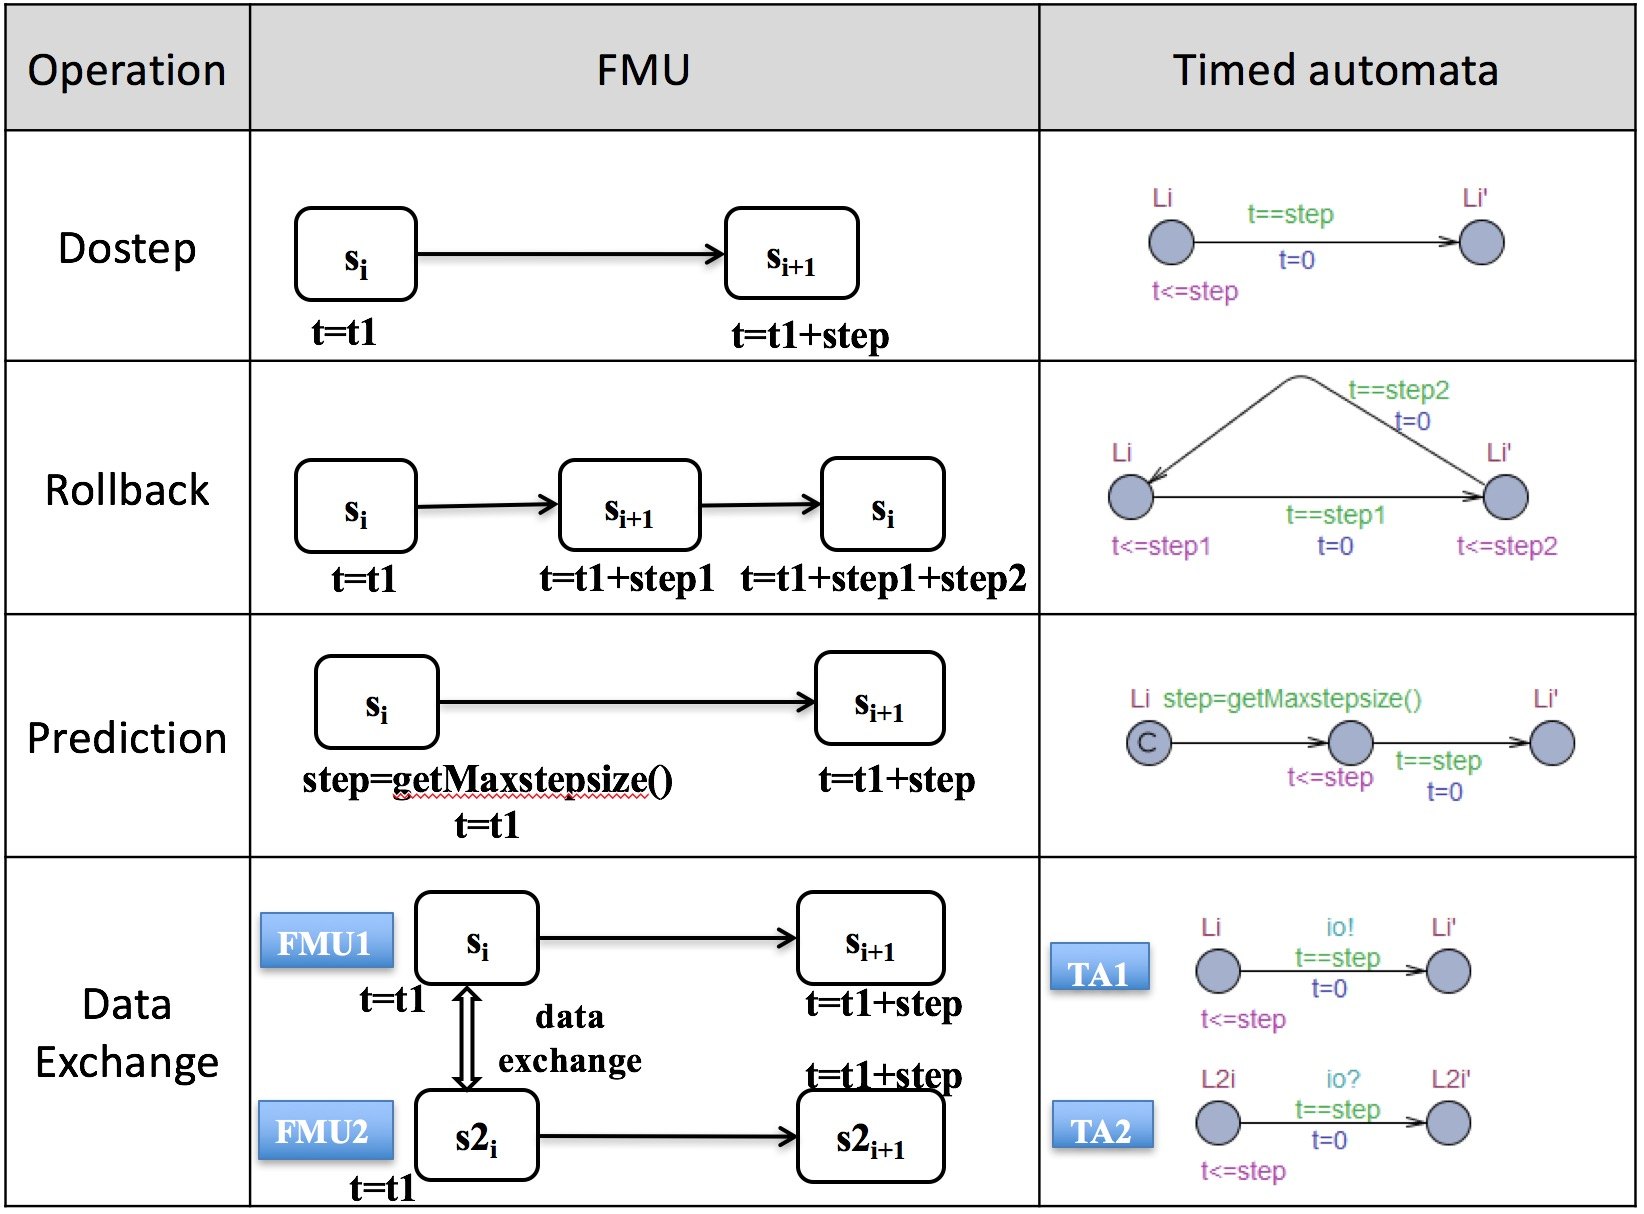
\includegraphics[width=3.5in,height=2.5in]{fig/abstractRole.png}}
	\caption{Encoding rules from FMU to TA.}
	\label{fmutota}
\end{figure}

It is not easy to translate FMU to TA directly, we propose some encoding rules from FMU to TA. As we can see in the Fig.\ref{fmutota}, given a state $s_{i}$ at $t_{1}$ in FMU, the operation $Dostep$ makes FMU reach a new state $s_{i+1}$ at $t_{1}+step$. This situation can be encoded into a transition in TA, in which a location $L_{i}$ delays $step$ time and goes to a new location $L_{i}^{\prime}$.

For the operation $Rollback$, given a state $s{i}$ at $t_{1}$ in FMU, the FMU will do a step1 to $s_{i+1}$ at $t_{1}+step1$, and then, the operation $rollback$ makes FMU reach the former state $s_{i}$. For this situation, it can be encoded as: location $L_{i}$ delays step1 time and reach a new location $L_{i}^{\prime}$ after a transition, next returns to the former Location $L_{i}$. 

For the operation $prediction$, given a state $s_{i}$, FMU can get max step size ($step$) for next step, and then reach a new state $s_{i+1}$ at $t_{1}+step$. For TA, it gets max step size in location $L_{i}$, then it delays $step$ time and reach a new location $L_{i}^{\prime}$ .

For data exchange between two FMUs in state $s_{i}$ at $t_{1}$, they exchange data at $t_{1}$ and then do the same step to $s_{i+1}$. In TA, there will be a signal $io$ to make the two FMUs do the same step from $L_{i}$ to $L_{i+1}$ after data exchange.

Although there are semantic gaps between FMUs and timed automata, we provide appropriate encoding rules to formalism FMU with timed automata. It lays the foundation for analyse FMI co-simulation with timed automata-based model checking.


